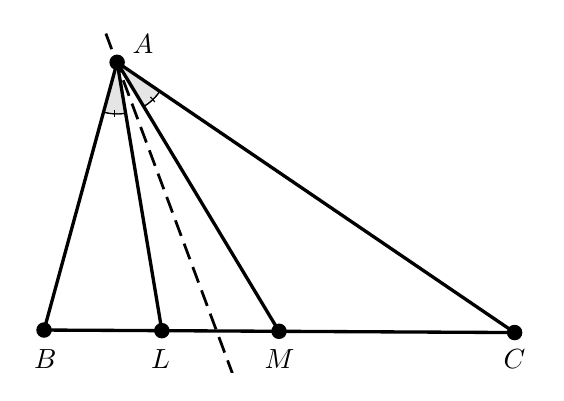
\begin{tikzpicture}[scale = 0.8]
    \clip(-2.58,-1.22) rectangle (5.48,4.26);
    \draw [shift={(-1.16,3.71)},fill=black,fill opacity=0.1] (0,0) -- (-105.3:0.82) arc (-105.3:-80.57:0.82) -- cycle;
    \draw [shift={(-1.16,3.71)},fill=black,fill opacity=0.1] (0,0) -- (-58.95:0.82) arc (-58.95:-34.22:0.82) -- cycle;
    \draw [line width=1.2pt] (-1.16,3.71)-- (-2.32,-0.54);
    \draw [line width=1.2pt] (-2.32,-0.54)-- (5.15,-0.58);
    \draw [line width=1.2pt] (-1.16,3.71)-- (5.15,-0.58);
    \draw [line width=1pt,dash pattern=on 6pt off 3pt,domain=-2.58:5.48] plot(\x,{(--0.2-0.94*\x)/0.35});
    \draw [line width=1.2pt] (-1.16,3.71)-- (-0.45,-0.55);
    \draw [line width=1.2pt] (-1.16,3.71)-- (1.41,-0.56);
    \draw [shift={(-1.16,3.71)}] (-105.3:0.82) arc (-105.3:-80.57:0.82);
    \draw(-1.2,2.95) -- (-1.2,2.84);
    \draw [shift={(-1.16,3.71)}] (-58.95:0.82) arc (-58.95:-34.22:0.82);
    \draw(-0.63,3.16) -- (-0.56,3.08);
    \begin{scriptsize}
        \normalsize
        \fill [color=black] (-1.16,3.71) circle (3.5pt);
        \draw[color=black] (-0.75, 4) node {$A$};
        \fill [color=black] (-2.32,-0.54) circle (3.5pt);
        \draw[color=black] (-2.3,-1) node {$B$};
        \fill [color=black] (5.15,-0.58) circle (3.5pt);
        \draw[color=black] (5.15,-1) node {$C$};
        \draw[color=black] (-1.79,6.02) node {$d$};
        \fill [color=black] (1.41,-0.56) circle (3.5pt);
        \draw[color=black] (1.42,-1) node {$M$};
        \fill [color=black] (-0.45,-0.55) circle (3.5pt);
        \draw[color=black] (-0.47,-1) node {$L$};
    \end{scriptsize}
\end{tikzpicture}